\documentclass[border=10pt]{standalone}

\usepackage{tikz}
\usepackage{tikzsymbols}
\usetikzlibrary{calc,patterns,shapes.geometric}

\def\centerarc[#1](#2)(#3:#4:#5){\draw[#1] ($(#2)+({#5*cos(#3)},{#5*sin(#3)})$) arc (#3:#4:#5);}

\begin{document}
	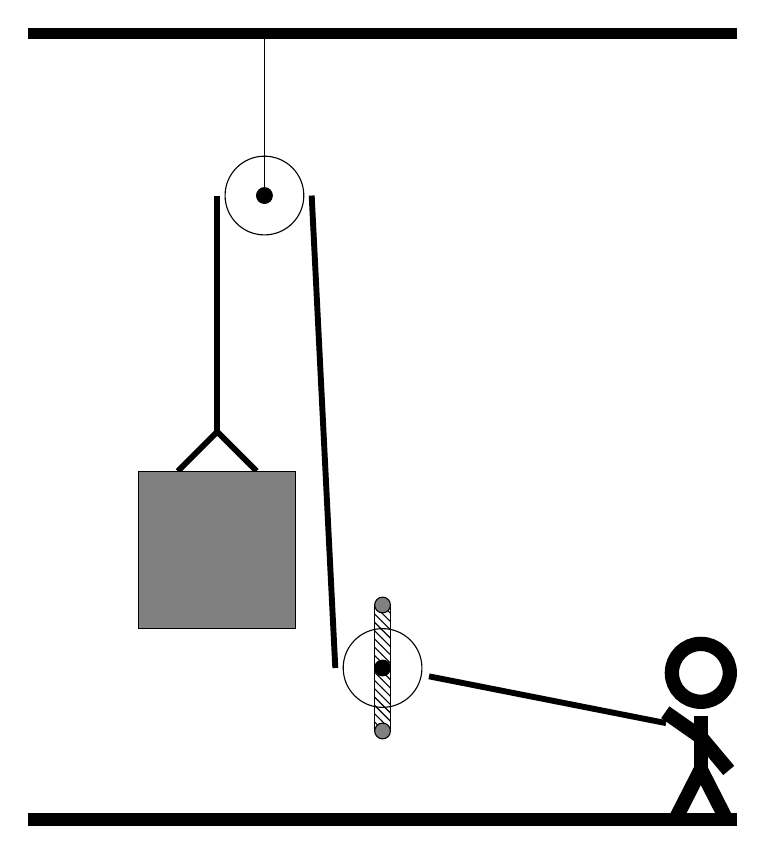
\begin{tikzpicture}
		%%%%% START %%%%%
		\draw[fill=black] (-2, 10) rectangle (7, 10.125);
		
		\draw (1, 8) circle (0.5);
		\draw[fill=black] (1, 8) circle (0.1);
		\draw (1, 10) -- (1, 8);
		
		\draw[fill=white](2.5, 2.0) circle (0.5);
		\draw[fill=black] (2.5, 2.0) circle (0.1);
		\draw[pattern=north west lines, pattern color=black] (2.4, 2.8) rectangle (2.6, 1.2);
		\draw[fill=black!50] (2.5, 2.8) circle (0.1);
		\draw[fill=black!50] (2.5, 1.2) circle (0.1);
		
		\draw[line width=0.75mm] (-0.1, 4.5) -- (0.4, 5.0) -- (0.9, 4.5);
		\draw[fill=black!50] (-0.6, 4.5) rectangle (1.4, 2.5);
		
		\draw[line width=0.75mm] (0.4, 8) -- (0.4, 5.0);
		\centerarc[line width=0.75mm](1, 8)(0:180:0.6);
		\draw[line width=0.75mm](1.6, 8) -- (1.9, 2.0);
		\centerarc[line width=0.75mm](2.5, 2.0)(180:270:0.6);
		\draw[line width=0.75mm](3.09, 1.894) -- (6.1, 1.3);
		
		\node at (6.5, 1.2) {\Strichmaxerl[10][-35][-50]};
		
		\draw[fill=black] (-2, 0) rectangle (7, 0.15);
		%%%%% END %%%%%
	\end{tikzpicture}
\end{document}